% ===================================================================
% Arquivo: capitulos/parte-III-pilares/cap-10-perda-binaria.tex
% ===================================================================

\chapter{Funções de Perda para Classificação}
\label{cap:perda-classificacao}

\section{Exemplo Ilustrativo:}

\section{Funções de Perda para Classificação Binária}

\subsection{Entropia Cruzada Binária (Binary Cross-Entropy - BCE): A função de perda padrão}

Para entender a função de perda \textit{Binary Cross Entropy} (\textit{BCE}) é importante antes conhecer o conceito de Entropia, o qual é fundamental para o cálculo dessa função. Em \textit{A Matematical Theory of Comunication}, \textcite{EntropyShannon} estava estudando sobre formas eficientes de comunicação, para isso, em um dos momentos do artigo ele define o conceito de Entropia, sendo uma medida de incerteza, ou da "escolha", associada a um conjunto de eventos com determinada probabilidades. Essa fórmula pode ser vista na Equação \ref{eq:entropia-de-shannon}.

\begin{equacaodestaque}{Entropia de Shannon}
    H(p) = - k \sum_{i = 1}^{n} p_i \log pi
    \label{eq:entropia-de-shannon}
\end{equacaodestaque}

Passado alguns anos, outros autores já estavam trabalhando com esse conceito introduzido por Shannon. Um desses casos é o de \textcite{KullbackLeiblerDivergence}, que em \textit{On Information and Sufficiency} expandem o conceito de Entropia para lidar também com casos contínuos, mas, mais que isso, introduzem uma media para comparar duas distribuições de probabilidades $p$ e $q$, chamando-a de informação para discriminação. Essa medida futuramente passa a ser conhecida com divergência de Kullback-Leibler (\textit{KL Divergence}), ela está representada na Equação \ref{eq:kl-divergence}

\begin{equacaodestaque}{Divergência de Kullback-Leibler}
    I(1:2) = I_{1:2}(X) = \int f_1 (x) \log \frac{f_1(x)}{f_2 (x)} d \lambda (x)
    \label{eq:kl-divergence}
\end{equacaodestaque}

Essa função tem como principal objetivo mediar a "perda" ou o "excesso" de informação quando é utilizada uma distribuição $q$ para aproximar a distribuição real $q$. Além disso, é a partir dessa fórmula que é possível chegar na definição de Entropia-Cruzada (\textit{Cross-Entropy}), para isso, o primeiro passo, é utilizar as propriedades do logarítmo para reescrever da divergência KL, assim, tem-se:

\[
    I(1:2) = I_{1:2}(X) = \int f_1 (x) (\log f_1 (x) - \log f_2 (x)) d\lambda (x)
\]

Em seguida, deve-se expandir a equação, utilizando a propriedade distributiva, encontrando então:

\[
    I(1:2) = I_{1:2}(X) = \int f_1 (x) \log f_1 (x) - f_1 (x) \log f_2 (x) d \lambda (x)
\]

A partir dessa nova equação, o próximo passo é separar a integral em duas diferentes, chegando na expressão:

\[
    I(1:2) = \int f_1 (x) \log f_1 (x) d\lambda (x) - \int f_1 (x) \log f_2 (x) d\lambda(x)
\]

Note que o primeiro termo é quase igual a fórmula proposta por Shannon para a Entropia, exceto por um sinal de menos, assim, o primeiro termo pode ser reescrito como $-H(f_1)$. Já o segundo termo é a própria definição de Entropia-Cruzada entre $f_1$ e $f_2$, portanto $H(f_1, f_2)$, o qual pode ser visto separadamente na Equação \ref{eq:cross-entropy}.

\begin{equacaodestaque}{Entropia-Cruzada (\textit{Cross-Entropy})}
    H(f_1, f_2) = \int f_1 (x) \log f_2 (x) d\lambda(x)
    \label{eq:cross-entropy}
\end{equacaodestaque}

Com base nesses dois termos, o da Entropia-Cruzada, e o da Entropia de Shannon, é possível mais uma vez reescrever a definição de xx agora utilizando os termos resumidos:

\[
    I(1:2) = H(f_1, f_2) - H(f_2)
\]

Ou também pode ser escrita como:

\[
    D_{KL} (f_1 || f_2) = H(f_1, f_2) - H(f_1)
\]

Portanto, é possível dizer que a Divergência de Kullback-Leibler é a diferença entre a Entropia-Cruzada e a Entropia de Shannon. Reescrevendo a equação mais uma vez é possível chegar em:

\[
    H(f_1, f_2) = H(f_1) + I(1:2)
\]

Essa equação nos diz que o custo real de codificar os dados usando um modelo imperfeito $H(f_1, f_2)$ é igual ao csuto de codificar usando um modelo perfeito $H(f_1)$ mais uma penalidade extra pela diferença entre o modelo perfeito e imperfeito. Assim, é possível concluir que ao minimizar a Divergência KL, é o mesmo que minimizar a Entropia-Cruzada em cenários de aprendizado de máquina. Isso se dá pois como a Entropia dos dados reais é uma constante, ao reduzir a Entropia-Cruzada, é ao mesmo tempo forçar a redução da Divergência KL, isso aproxima mais o modelo dos dados da realidade.

A partir desses dois conceitos é possível conhecer melhor a função de perda \textit{Binary-Cross-Entropy}. Ela é dada pela Equação \ref{eq:binary-cross-entropy}. Note, que a definição da \textit{BCE} apresente grandes similaridades com Entropia-Cruzada, principalmente pelos primeiros termos $y \log (\hat{y})$, que é justamente a definição de Entropia-Cruzada.

\begin{equacaodestaque}{Entropia Cruzada Binária}
    L(y, \hat{y}) = -[y \log(\hat{y}) + (1 - y) \log(1 - \hat{y})]
    \label{eq:binary-cross-entropy}
\end{equacaodestaque}

Além disso, a \textit{BCE} já vem sendo utilizada no contexto de aprendizado de máquina a um bom tempo. Um dos trabalhos que cita o uso dessa função para ser utilizada em cenários de classificação binária é o \textit{Connectionist Learning Procedures} de \textcite{HintonConnectionist}, em que o autor cita que ao minimizar a Entropia-Cruzada-Binária para as distribuições do resultado desejado e o atual resultado era semelhante a maximivizar a a versossimilhança do modelo gerar as saídas corretas.

Dito isso, o próximo passo para entender a \textit{BCE} é conhecer a sua representação gráfica, a qual está presente na Figura \ref{fig:binary-cross-entropy}. Note que o gráfico apresenta duas curvas, uma para a distribuição para a classe real, e outra para a distribuição para a classe de saídas do modelo. Perceba que o ponto de mínimo do gráfico é aquele em que as duas curvas se encontram, e com isso a distância entre as duas é mínima, e consequentemente a perda também será.

\begin{figure}
    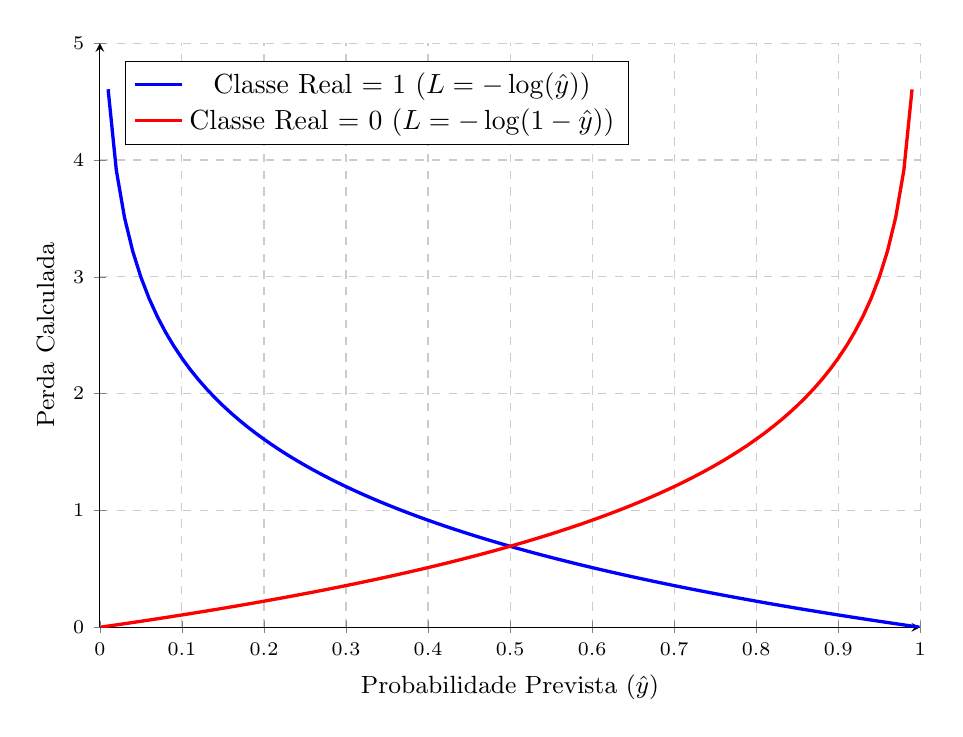
\begin{tikzpicture}
        \begin{axis}[
            xlabel={Probabilidade Prevista ($\hat{y}$)},
            ylabel={Perda Calculada},
            axis lines=left,              % Eixos no canto inferior esquerdo
            grid=major,                   % Adiciona uma grade principal
            grid style={dashed, gray!40},   % Estilo da grade
            xmin=0, xmax=1,               % Limites do eixo x
            ymin=0, ymax=5,               % Limites do eixo y
            legend pos=north west,      % Posição da legenda
            width=12cm,                   % Largura do gráfico
            height=9cm,                   % Altura do gráfico
            title style={font=\bfseries},
            label style={font=\small},
            tick label style={font=\scriptsize}
        ]
            % Curva para a classe real y=1
            \addplot[
                domain=0.01:0.999, % Domínio para evitar log(0)
                samples=100,
                color=blue,
                very thick
            ] {-ln(x)};
            \addlegendentry{Classe Real = 1 ($L = -\log(\hat{y})$)}

            % Curva para a classe real y=0
            \addplot[
                domain=0.001:0.99, % Domínio para evitar log(0)
                samples=100,
                color=red,
                very thick
            ] {-ln(1-x)};
            \addlegendentry{Classe Real = 0 ($L = -\log(1-\hat{y})$)}
            
        \end{axis}
    \end{tikzpicture}
    \caption{Representação gráfica da função de perda Entropia-Cruzada-Binária (\textit{Binary-Cross-Entropy}).}
    \label{fig:binary-cross-entropy}
    \fonte{O autor (2025).}
\end{figure}

\begin{equacaodestaque}{Derivada da Entropia Cruzada Binária}
    \frac{\partial L}{\partial \hat{y}} = \frac{\hat{y} - y}{\hat{y}(1 - \hat{y})}
    \label{eq:binary-cross-entropy-derivada}
\end{equacaodestaque}

\subsection{Perda Hinge (Hinge Loss)}

\begin{equacaodestaque}{Hinge Loss}
    L(y, f(x)) = \max(0, 1 - y \cdot f(x))
    \label{eq:hinge-loss}
\end{equacaodestaque}

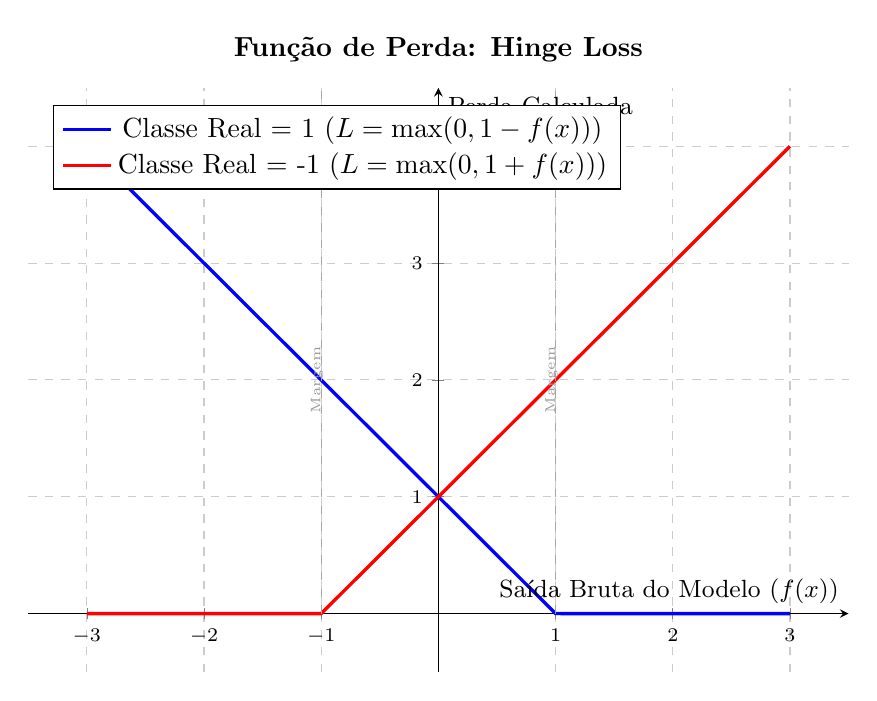
\begin{tikzpicture}
    \begin{axis}[
        title={Função de Perda: Hinge Loss},
        xlabel={Saída Bruta do Modelo ($f(x)$)},
        ylabel={Perda Calculada},
        axis lines=middle,          % Eixos centrados em (0,0)
        grid=major,                 % Adiciona uma grade principal
        grid style={dashed, gray!40}, % Estilo da grade
        xmin=-3.5, xmax=3.5,        % Limites do eixo x
        ymin=-0.5, ymax=4.5,         % Limites do eixo y
        legend pos=north west,      % Posição da legenda
        width=12cm,                 % Largura do gráfico
        height=9cm,                 % Altura do gráfico
        title style={font=\bfseries},
        label style={font=\small},
        tick label style={font=\scriptsize}
    ]
        % Curva para a classe real y=+1
        \addplot[
            domain=-3:3, 
            samples=100, 
            color=blue, 
            very thick
        ] {max(0, 1-x)};
        \addlegendentry{Classe Real = 1 ($L=\max(0, 1-f(x))$)}

        % Curva para a classe real y=-1
        \addplot[
            domain=-3:3, 
            samples=100, 
            color=red, 
            very thick
        ] {max(0, 1+x)};
        \addlegendentry{Classe Real = -1 ($L=\max(0, 1+f(x))$)}
        
        % Opcional: Linhas tracejadas para marcar as margens
        \draw[dashed, gray!70] (axis cs:1, 0) -- (axis cs:1, 4.5);
        \draw[dashed, gray!70] (axis cs:-1, 0) -- (axis cs:-1, 4.5);
        \node[above, gray!80, font=\tiny, rotate=90] at (axis cs:1.1, 2) {Margem};
        \node[above, gray!80, font=\tiny, rotate=90] at (axis cs:-0.9, 2) {Margem};
        
    \end{axis}
\end{tikzpicture}

\begin{equacaodestaque}{Derivada da Hinge Loss}
    \frac{\partial L}{\partial f(x)} = 
    \begin{cases} 
      -y & \text{se } y \cdot f(x) < 1 \\
      0 & \text{se } y \cdot f(x) \ge 1
    \end{cases}
    \label{eq:hinge-loss-derivada}
\end{equacaodestaque}

\section{Funções de Perda para Classificação Multilabel}

\subsection{Entropia Cruzada Categórica (Categorical Cross-Entropy)} 

\begin{equacaodestaque}{Entropia Cruzada Categórica}
    L(y, \hat{y}) = - \sum_{c=1}^{C} y_c \log(\hat{y}_c)
    \label{eq:categorical-cross-entropy}
\end{equacaodestaque}

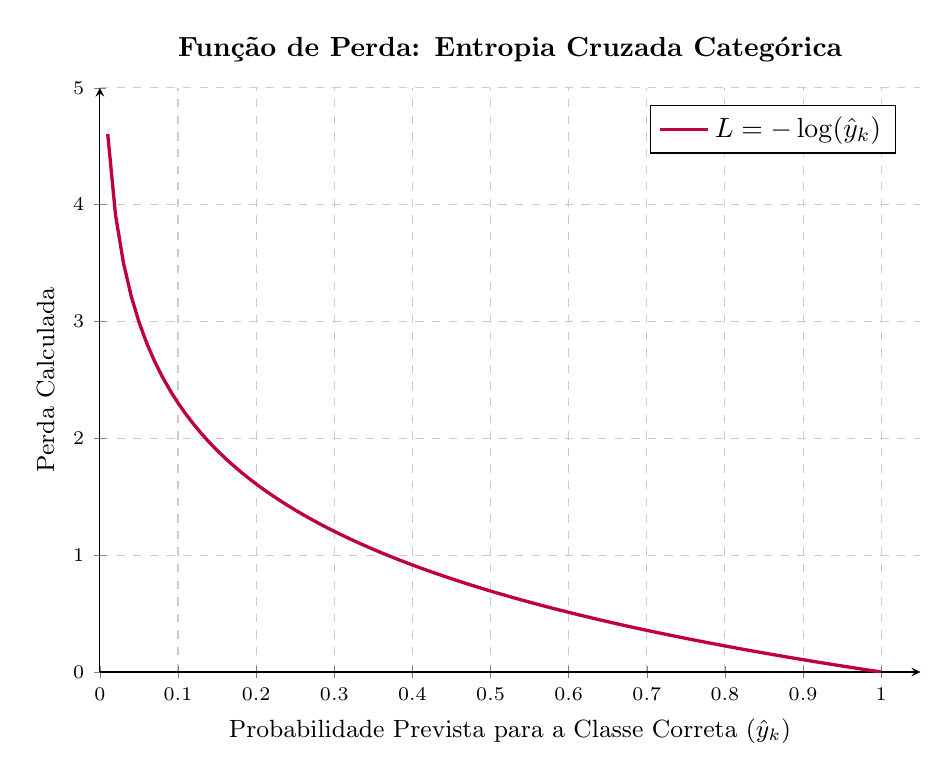
\begin{tikzpicture}
    \begin{axis}[
        title={Função de Perda: Entropia Cruzada Categórica},
        xlabel={Probabilidade Prevista para a Classe Correta ($\hat{y}_k$)},
        ylabel={Perda Calculada},
        axis lines=left,              % Eixos no canto inferior esquerdo
        grid=major,                   % Adiciona uma grade principal
        grid style={dashed, gray!40},   % Estilo da grade
        xmin=0, xmax=1.05,            % Limites do eixo x
        ymin=0, ymax=5,               % Limites do eixo y
        legend pos=north east,        % Posição da legenda
        width=12cm,                   % Largura do gráfico
        height=9cm,                   % Altura do gráfico
        title style={font=\bfseries},
        label style={font=\small},
        tick label style={font=\scriptsize}
    ]
        % Plota a função -log(y_k_hat)
        \addplot[
            domain=0.01:1, % Domínio para evitar log(0)
            samples=100,
            color=purple,
            very thick
        ] {-ln(x)};
        
        \addlegendentry{$L = -\log(\hat{y}_k)$}
        
    \end{axis}
\end{tikzpicture}

\begin{equacaodestaque}{Derivada da Entropia Cruzada Categórica}
    \frac{\partial L}{\partial z_i} = \hat{y}_i - y_i
    \label{eq:category-cross-entropy-derivada}
\end{equacaodestaque}

\subsection{Entropia Cruzada Categórica Esparsa (Sparse Categorical Cross-Entropy)}

\begin{equacaodestaque}{Entropia Cruzada Categórica Esparsa}
    L_i = - \log(\hat{y}_{i, y_i})
    \label{eq:sparse-categorical-cross-entropy}
\end{equacaodestaque}

\begin{equacaodestaque}{Derivada da Entropia Cruzada Categórica Esparsa}
    \frac{\partial L_i}{\partial z_{i,k}} = \hat{y}_{i,k} - y_{i,k}
    \label{eq:sparse-categorical-cross-entropy-derivada}
\end{equacaodestaque}

\section{Comparativo: Funções de Perda para Classificação}

\section{Fluxograma: Escolhendo a Função de Perda Ideal}